 \documentclass[14pt]{beamer}
\usepackage[T1]{fontenc} 
\usepackage[utf8]{inputenc}
\usepackage[french]{babel}
\usepackage{color}

\setbeamertemplate{blocks}[rounded]

\usetheme{CambridgeUS}
\hypersetup{
  colorlinks,
  citecolor=black,
  filecolor=black,
  linkcolor=black,
  urlcolor=black
}

\title{Logoot}
\subtitle{a Scalable Optimistic Replication Algorithm for Collaborative Editing on P2P Networks}
\author{Adrien Drouet\\
        Alexandre Prenza}

\begin{document}
  %%%%%%%%%%%%%%%%%%%%%%%%%%%%%%%%%%%%%%%%%%%%%%%%%%%%%%%%%%%%%%%%%%%%%%%%%%%%%%
  %% Titre
  %%%%%%%%%%%%%%%%%%%%%%%%%%%%%%%%%%%%%%%%%%%%%%%%%%%%%%%%%%%%%%%%%%%%%%%%%%%%%%
  \begin{frame}
    \titlepage
  \end{frame}

	\begin{frame}
		\frametitle{Introduction}
		\begin{itemize}
			\item<1-> Collaborative editing
			\item <2->Wikipedia
				\begin{itemize}
					\item<3-> 10 million of articles
					\item<3-> Centralized infrastructure
					\begin{itemize}
						\item<4-> Poor fault tolerance
						\item<4-> Costly scalability
					\end{itemize}
				\end{itemize}
			\item<5-> Solution ?
			\begin{itemize}
						\item<6-> Peer-to-peer
			\end{itemize}
		\end{itemize}
	\end{frame}

	\begin{frame}
		\frametitle{P2P}
		Peer-to-Peer constraint
		\begin{itemize}
			\item Churn - Peers which enter and leave the network
			\item Unknow/unbouded set of peer
		\end{itemize}
		
		Collaborative and real-time editor must insure the CCI :
		\begin{itemize}
			\item<2-> Causality : Ensure all operations are ordered
			\item<2-> Convergence : Convergence of the system when idle
			\item<2-> Intention : Expected effect observed on all replica
			\item<2-> Scalability : Must handle addition of users or objects
		\end{itemize}
	\end{frame}

	\begin{frame}
	  \frametitle{Related Work}
		\begin{itemize}
			\item<1-> WOOKI : Hasse diagramm extension
			\begin{itemize}
				\item<1-> P2P system
				\item<1-> Barely respect CCI
				\item<1-> Use tombstones
			\end{itemize}
			\item<2-> TreeDoc : Binary tree
			\begin{itemize}
				\item<2-> P2P system
				\item<2-> Use tombstones
				\item<2-> Proposed procedure to remove tombstones but cannot be used in P2P
			\end{itemize}			
		\end{itemize}
	\end{frame}

	\begin{frame}
		\frametitle{Proposition}
		\begin{itemize}
			\item Logoot
			\begin{itemize}
				\item Linear structure
				\item Total order between elements
				\item Any element (line) as an unique identifier
			\end{itemize}
			\item Two operations
			\begin{itemize}
				\item Insert(pid,text)
				\item Delete(pid)
			\end{itemize}
		\end{itemize}
	\end{frame}

	\begin{frame}
		\frametitle{Logoot model - Identifier}
		Identifier
		\begin{itemize}
			\item Couple (pid, content)
			\item $pid=pid_1.pid_2...pid_n.(pos, site)$
			\item Total order :
				\begin{itemize}
					\item $(1,1) < (1,3)$
					\item $(1,1)(5,2) < (1,1)(14,1) < (4,2) $
				\end{itemize}
		\end{itemize}		
	\end{frame}

	\begin{frame}
		\frametitle{Logoot model - Identifier}
		\begin{itemize}
			\item<1-> \emph{(0,0)} - Begining of the document
			\item<2-> \emph{(1,1),0} - Line 1 insered
			\item<4-> \emph{(1,1)(1,5),4} - Line 3 insered between line 1 and line 2
			\item<3-> \emph{(1,3),2} - Line 2 insered
			\item<1-> \emph{(MAX,0)} - End of the document
		\end{itemize}		
	\end{frame}

	\begin{frame}
		\frametitle{Logoot model - Modifying and Integrating}
		\begin{itemize}
			\item Modifying
				\begin{itemize}
					\item Generate one or more identifier
					\item Postion can become bigger
				\end{itemize}
			\item Integration
				\begin{itemize}
					\item Binary search
					\item Logarithmic time
					\item Deletion doesn't need tombstone to insure convergence
				\end{itemize}		
		\end{itemize}
	\end{frame}

	\begin{frame}
		\frametitle{Result}
		\begin{itemize}
			\item Methodology
				\begin{itemize}
					\item Wooto, TreeDoc and Logoot
					\item Most edited encyclopedic pages
					\item Most edited pages
					\item Biggest pages
					\item Over the last 100 edits
				\end{itemize}
			\item Observation of overhead
		\end{itemize}
		
	\end{frame}

	\begin{frame}
		\frametitle{Result}
			Experimentation : Most edited encyclopedic pages
			\begin{figure}
				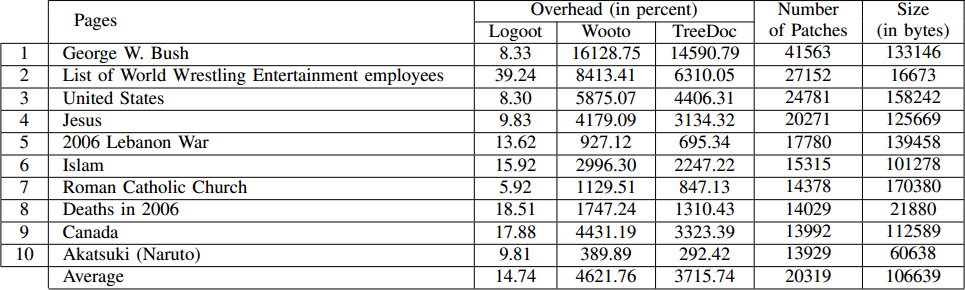
\includegraphics[width=1\textwidth]{includes/etu1}
			\end{figure}
	\end{frame}

	\begin{frame}
		\frametitle{Result}
			Experimentation : Most edited pages
			\begin{figure}
				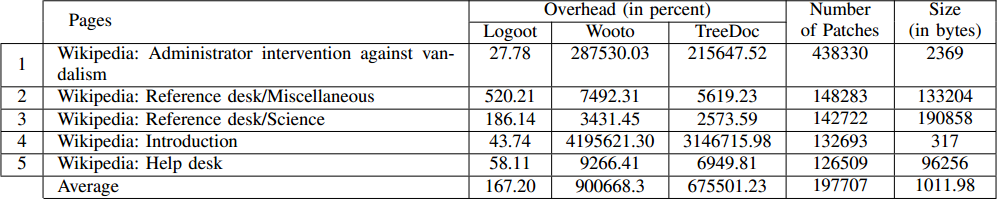
\includegraphics[width=1\textwidth]{includes/etu2}
			\end{figure}
	\end{frame}

	\begin{frame}
		\frametitle{Result}
			Experimentation : Biggest pages
			\begin{figure}
				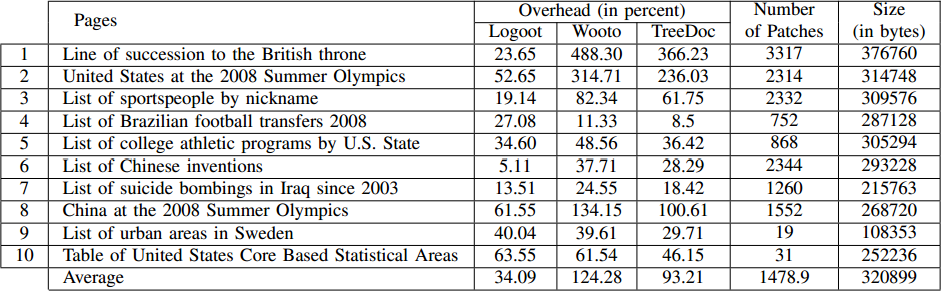
\includegraphics[width=1\textwidth]{includes/etu3}
			\end{figure}
	\end{frame}

	\begin{frame}
		\frametitle{Result}
			Logoot observation :
			\begin{itemize}
				\item Relative overhead seem constant
				\item Way better when number of patch > 10.000 
				\item A little better when number of patch < 2.000
			\end{itemize}
			Why ?
			\begin{itemize}
				\item No tombstones to maintain order
				\item A lot of deletion (Update = Delete + Insert)
			\end{itemize}
	\end{frame}

	\begin{frame}
		\frametitle{Conclusion}
			\begin{itemize}
				\item Logoot ensure the CCI on P2P network
				\item It does not require tombstones
				\item Space overhead remains linear
				\item Better performances than WOOT and Treedoc
			\end{itemize}
	\end{frame}

\end{document}

